% ==============================================================================
% condensed_results.tex
%
% Condensed Methods + Results chapter for the DermaMNIST federated-learning
% thesis. Short paragraphs, three-decimal numbers, direct declarative prose,
% one master summary table.
%
% Target length: approximately 5,500 words (Methods ~1,000, Results ~4,500).
%
% This file compiles standalone (\documentclass...\end{document}) for preview,
% and can also be \input'd into the main thesis after stripping the preamble.
% ==============================================================================

\documentclass[11pt,a4paper]{report}

\usepackage[utf8]{inputenc}
\usepackage[T1]{fontenc}
\usepackage{graphicx}
\graphicspath{{mnist_dermnist/results/thesis_ready/figures/}}
\usepackage{booktabs}
\usepackage{amsmath, amssymb}
\usepackage{bm}
\usepackage{microtype}

\usepackage{hyperref}
\usepackage{caption}
\usepackage{xcolor}
\usepackage[margin=2.5cm]{geometry}
\usepackage{setspace}
\usepackage[round,authoryear]{natbib}
\onehalfspacing

\title{Federated Optimisation on DermaMNIST\\
\large Condensed Methods and Results}
\author{Barbara Koch}
\date{}

\begin{document}

\maketitle

% ==============================================================================
\chapter{Methods}
\label{ch:methods-condensed}
% ==============================================================================

\section{Dataset}
\label{sec:cond-dataset}

DermaMNIST is the dermatoscopic image classification subset of MedMNIST v2
\citep{yang2023medmnistv2}, derived from the HAM10000 collection
\citep{tschandl2018ham10000}. It comprises $10{,}015$ RGB skin-lesion images
resized to $28 \times 28$ pixels and labelled into seven diagnostic classes.
The class distribution is severely imbalanced: melanocytic nevi (mel-nevi)
accounts for $66.9\%$ of the test set ($1{,}341 / 2{,}005$), while
dermatofibroma and vascular lesions account for $1.1\%$ and $1.4\%$
respectively. The official MedMNIST train/validation/test split
($7{,}007/1{,}003/2{,}005$) is preserved throughout.

\section{Model and Training}
\label{sec:cond-model}

A compact $7$-class CNN with three $3 \times 3$ convolutional blocks
(GroupNorm, ReLU, max-pool) followed by a $128$-unit fully-connected layer is
used as the shared client and global model. Local training uses SGD with
momentum $0.9$, weight decay $10^{-4}$, learning rate $0.01$, batch size $64$,
and $E = 20$ local epochs per round. Federated training runs for $R = 150$
communication rounds. Test metrics are reported at the best-validation
checkpoint round unless stated otherwise.

\section{Federated Setup and Algorithms}
\label{sec:cond-fl}

The federation comprises $K = 2$ clients in the main experiments (with one
$7$-client case study in Section~\ref{sec:cond-small-hospital}). The training
data is partitioned across clients to simulate four heterogeneity scenarios
described in Section~\ref{sec:cond-stat-het}: IID, Dirichlet ($\alpha = 0.1$),
specialist-by-class, and an engineered $90/10$ split with rare-class
redistribution. Three federated optimisers are compared:

\paragraph{FedAvg \citep{mcmahan2017fedavg}} aggregates client weights as a
sample-size-weighted average each round.

\paragraph{FedProx \citep{li2020fedprox}} adds a proximal term
$\frac{\mu}{2}\Vert w - w^{(t)} \Vert^2$ to each client's local loss
($\mu = 0.01$ as the default), and accepts partial updates from stragglers
under the $\gamma$-inexact framework.

\paragraph{FedNova \citep{wang2020fednova}} rescales each client's update by
its number of completed local steps ($\tau_i$-normalisation) before averaging,
intended to correct the objective inconsistency caused by unequal local
training.

System heterogeneity is modelled in two complementary ways. The
\emph{straggler} protocol (Section~\ref{sec:cond-system-het}), following
\citet{li2020fedprox} §5.2, marks a fraction $X$ of clients as stragglers each
round and assigns them a random partial-completion fraction
$\gamma_k \sim \mathrm{Uniform}(0, 1)$. The \emph{unequal-$E$} and
\emph{unequal-learning-rate} protocols
(Section~\ref{sec:cond-lr-asymmetry}) hold all clients in the round but assign
them different per-client local-epoch counts or learning rates.

\section{Evaluation and Reporting Protocol}
\label{sec:cond-evaluation}

Multi-class macro-F1 over the seven DermaMNIST test classes is the primary
metric, chosen over accuracy because the $66.9\%$ mel-nevi dominance renders
accuracy uninformative. The paired-seed protocol of \citet{li2020fedprox} is
used for the headline 10-seed comparisons: each comparison sets the same
PyTorch and NumPy seeds for both algorithms, so that within-pair differences
isolate algorithmic effect from initialisation noise. Three-seed
multi-seed promotions ($\{42, 123, 456\}$) are used elsewhere unless
stated. All standard deviations are sample standard deviations
($\textnormal{ddof} = 1$). Pairwise statistical tests are paired Wilcoxon
signed-rank, two-sided.

\section{Implementation}
\label{sec:cond-implementation}

Experiments are implemented in PyTorch~$2.4$ and the Flower federated
simulation framework~$1.23$ \citep{beutel2020flower}, executed on Cambridge
HPC SLURM nodes. Code, history CSVs, predictions, and SLURM logs are
preserved under
\path{cleanest_federated/mnist_dermnist/results/} with provenance manifests in
\path{README_PROVENANCE.md} files per experiment directory.

% ==============================================================================
\chapter{Results and Discussion}
\label{ch:results-condensed}
% ==============================================================================

This chapter reports the empirical comparison of FedAvg, FedProx, and FedNova
on DermaMNIST across statistical and system heterogeneity. Section~\ref{sec:cond-baseline}
establishes the centralised and IID anchors; Section~\ref{sec:cond-engineered}
reports the headline 10-seed engineered-partition result;
Section~\ref{sec:cond-stat-het} shows that statistical heterogeneity alone
does not separate the algorithms; Sections~\ref{sec:cond-system-het} and
\ref{sec:cond-lr-asymmetry} characterise the two regimes of system asymmetry
that do; Section~\ref{sec:cond-rare-class} describes the rare-class
collapse failure mode common to the failures observed throughout;
Section~\ref{sec:cond-mechanism} examines per-client update norms;
Section~\ref{sec:cond-ablations} reports algorithmic ablations and
methodological audits; Section~\ref{sec:cond-summary} synthesises the
findings. Six headline findings are isolated and stated explicitly at the
end of their respective sections.

\section{Centralised and IID Baselines}
\label{sec:cond-baseline}

The centralised baseline, trained on the pooled training set for the same
$E \times R$ local-step budget used in federation, reaches a mean test
macro-F1 of $0.560 \pm 0.024$ across ten seeds. The IID federated baseline
(50/50 stratified two-client split) reaches $0.585 \pm 0.020$ for FedAvg and
$0.579 \pm 0.019$ for FedProx, with a within-pair $\Delta = -0.006$ and
FedProx winning $5/10$ paired seeds. The two algorithms are functionally
indistinguishable under matched data distributions, and the federation tax
(centralised minus best federated) is approximately $0.06$ macro-F1.

\section{Engineered Non-IID Partition: Primary Result}
\label{sec:cond-engineered}

The engineered two-client partition assigns $90\%$ of the training data to
Client~0 and $10\%$ to Client~1, with the four rarest classes
(dermatofibroma, melanoma, vascular, actinic keratoses) over-represented in
Client~1's small dataset. Across ten paired seeds, FedAvg reaches a mean test
macro-F1 of $0.477 \pm 0.025$ and FedProx reaches $0.503 \pm 0.014$, giving a
mean within-pair $\Delta = +0.027$ (paired Wilcoxon $p = 0.020$,
rank-biserial $r = +0.818$, bootstrap $95\%$ CI excluding zero). FedProx
wins $9/10$ paired seeds. Variance is markedly lower under FedProx: the
across-seed standard deviation is $0.014$ for FedProx versus $0.025$ for
FedAvg, a $45\%$ reduction.

The advantage is concentrated on minority classes. Mean class-level $\Delta$
F1 is $+0.114$ on melanoma (paired Wilcoxon $p = 0.006$) and $+0.067$ on
actinic keratoses ($p = 0.020$), corresponding to relative gains of $61\%$
and $17\%$ on the per-class F1 baseline. The majority class (mel-nevi) shows
$\Delta = -0.003$, within seed noise. The pre-registered safety criterion
that no class regress by more than $0.05$ F1 is satisfied with margin (the
worst regression is vascular at $-0.012$). Figure~\ref{fig:cond-engineered}
shows the mean validation trajectories and the per-class breakdown.

\begin{figure}[!htbp]
\centering

\includegraphics[width=0.95\textwidth]{F_engineered_convergence.pdf}
\caption{Validation macro-F1 across $150$ communication rounds for the
engineered partition, mean over ten paired seeds. FedProx is more stable
during training and converges to a higher final value.}
\label{fig:cond-engineered}
\end{figure}

\paragraph{Finding 1.}
\textit{FedProx improves test macro-F1 over FedAvg by $+0.027$ on a
two-client non-IID DermaMNIST partition (10 seeds, paired Wilcoxon
$p = 0.020$), with a $61\%$ relative gain concentrated on melanoma and a
$45\%$ reduction in across-seed variance.}

\section{Statistical Heterogeneity Across Partitions}
\label{sec:cond-stat-het}

The engineered-partition result is verified across three further
non-IID partition designs. Table~\ref{tab:cond-partition-robustness} reports
all four. Across the three non-IID designs the within-pair $\Delta$ is
consistently positive ($+0.007$ to $+0.008$) and FedProx wins the majority of
paired seeds; under IID the direction reverses to a non-significant
$\Delta = -0.006$. The pattern --- positive under non-IID, near-zero under
IID --- reproduces the qualitative motivation of the proximal-anchor
mechanism.

\begin{table}[!htbp]
\centering
\caption{Test macro-F1 across partition designs (10 paired seeds; mean
$\pm$ sample SD).}
\label{tab:cond-partition-robustness}
\small
\begin{tabular}{lcccc}
\toprule
Partition                       & FedAvg              & FedProx             & $\Delta$ & Wins   \\
\midrule
IID                              & $0.585 \pm 0.020$   & $0.579 \pm 0.019$   & $-0.006$ & $5/10$ \\
Dirichlet $\alpha = 0.1$         & $0.480 \pm 0.036$   & $0.488 \pm 0.034$   & $+0.008$ & $6/10$ \\
Specialist (1-of-7)              & $0.437 \pm 0.024$   & $0.445 \pm 0.017$   & $+0.008$ & $7/10$ \\
Engineered 90/10 (Section~\ref{sec:cond-engineered}) & $0.496 \pm 0.015$ & $0.503 \pm 0.021$ & $+0.007$ & $7/10$ \\
\bottomrule
\end{tabular}
\end{table}

The Dirichlet aggregate $\Delta = +0.008$ understates the typical case
because of a single catastrophic seed: at seed $8675309$, FedProx training
diverged to a final test macro-F1 of $0.114$ (versus FedAvg's $0.486$).
Excluding this seed gives Dirichlet $\Delta = +0.042$ with FedProx winning
$9/10$ seeds; the aggregate retains all ten seeds for transparency. Across
all partitions, the absolute non-IID effect magnitudes ($\sim +0.01$) are
comparable to the across-seed standard deviations ($0.02$--$0.04$), and we
report them as descriptive observations of direction rather than as
quantitatively distinguishable effects.

The heterogeneity ladder isolates components of non-IID design. Five
partitions of increasing severity (L0 IID, L1 quantity-only, L2 label-skew,
L3 mixed, L4 severe; Jensen--Shannon divergences $0.000$ to $0.385$) yield
FedProx-minus-FedAvg differences of $\{-0.003, +0.002, -0.012, -0.003,
-0.026\}$ in a single-seed pilot. No monotonic dose-response is observed.
Promotion of the L4 cell to three seeds and a single physical compute node
(to remove cross-node CUDA non-determinism as a confounder) yields FedAvg
$0.492 \pm 0.019$ and FedProx $0.486 \pm 0.019$, a $\Delta = -0.006$ that is
one-sixth of the pooled cross-seed standard deviation. Under reporting at
best-validation, final-round, and last-$25$-round mean, two of the three seeds
flip the algorithm ordering (Section~\ref{sec:cond-ablations}), strengthening
rather than weakening the null interpretation.

The proximal coefficient $\mu$ has a narrow operating range. Across partitions
$\{L0, L2, L4\}$ tested at $\mu \in \{0.001, 0.01, 0.1, 1.0\}$, the optimal
$\mu$ is small at every partition ($\mu = 0.001$ at L0 and L2; $\mu = 0.01$
at L4, with FedAvg still ahead). $\mu = 1.0$ produces the worst FedProx
result at every partition, with the deficit growing from $0.064$ macro-F1
below the best at L0 to $0.127$ below at L4. The literature prescription
that larger $\mu$ should be preferred under greater heterogeneity
\citep{li2020fedprox} is not supported on this benchmark.

\paragraph{Finding 2.}
\textit{Statistical heterogeneity alone --- even at Jensen--Shannon
divergence $0.385$ under the engineered L4 partition --- does not robustly
separate FedAvg from FedProx under the symmetric protocol on this
benchmark.}

\section{System Heterogeneity: the $\gamma$-Inexact Mechanism}
\label{sec:cond-system-het}

The FedProx vs FedAvg gap grows substantially once system asymmetry is
introduced. Following \citet{li2020fedprox} §5.2, $50\%$ of clients are
marked as stragglers each round and complete only a random fraction
$\gamma_k \in (0, 1)$ of $E = 20$ local epochs. FedAvg drops these partial
updates entirely; FedProx accepts them under the $\gamma$-inexact framework.
A four-condition decomposition isolates the proximal term from the
$\gamma$-inexact handling: Table~\ref{tab:cond-li2020} reports three seeds
per cell.

\begin{table}[!htbp]
\centering
\caption{Li 2020 §5.2 four-condition decomposition at L4 (3 seeds; mean
$\pm$ sample SD).}
\label{tab:cond-li2020}
\small
\begin{tabular}{lc}
\toprule
Condition                                            & Test macro-F1 \\
\midrule
FedAvg, no stragglers                                & $0.484 \pm 0.027$ \\
FedAvg + drop + straggler                            & $0.364 \pm 0.009$ \\
FedProx + drop + straggler (control)                 & $0.368 \pm 0.005$ \\
FedProx + $\gamma$-inexact + straggler $\bigstar$    & $\mathbf{0.479 \pm 0.010}$ \\
\bottomrule
\end{tabular}
\end{table}

The decomposition reads as follows. Adding $50\%$ stragglers to FedAvg with
drop-handling causes a $0.120$ macro-F1 drop ($0.484 \to 0.364$). Adding the
proximal term while keeping drop-handling recovers only $+0.004$ macro-F1
($0.364 \to 0.368$). Switching from drop to $\gamma$-inexact under FedProx
recovers an additional $+0.111$ ($0.368 \to 0.479$), restoring the global
model to within $0.005$ of the no-straggler baseline.

\textbf{The proximal term contributes essentially nothing to the headline
FedProx win under stragglers; $\gamma$-inexact partial-update handling
contributes almost all of it.} Figure~\ref{fig:cond-val-curves}A makes this
explicit: the FedAvg-drop and FedProx-drop trajectories overlap nearly
perfectly across all $150$ rounds, while FedProx-$\gamma$-inexact climbs
alongside the no-straggler baseline. The mechanism is information loss
versus information rescue: drop-handling under non-IID systematically loses
rare-class gradients from the dropped straggler, while $\gamma$-inexact
preserves them at reduced strength.

\begin{figure}[!htbp]
\centering
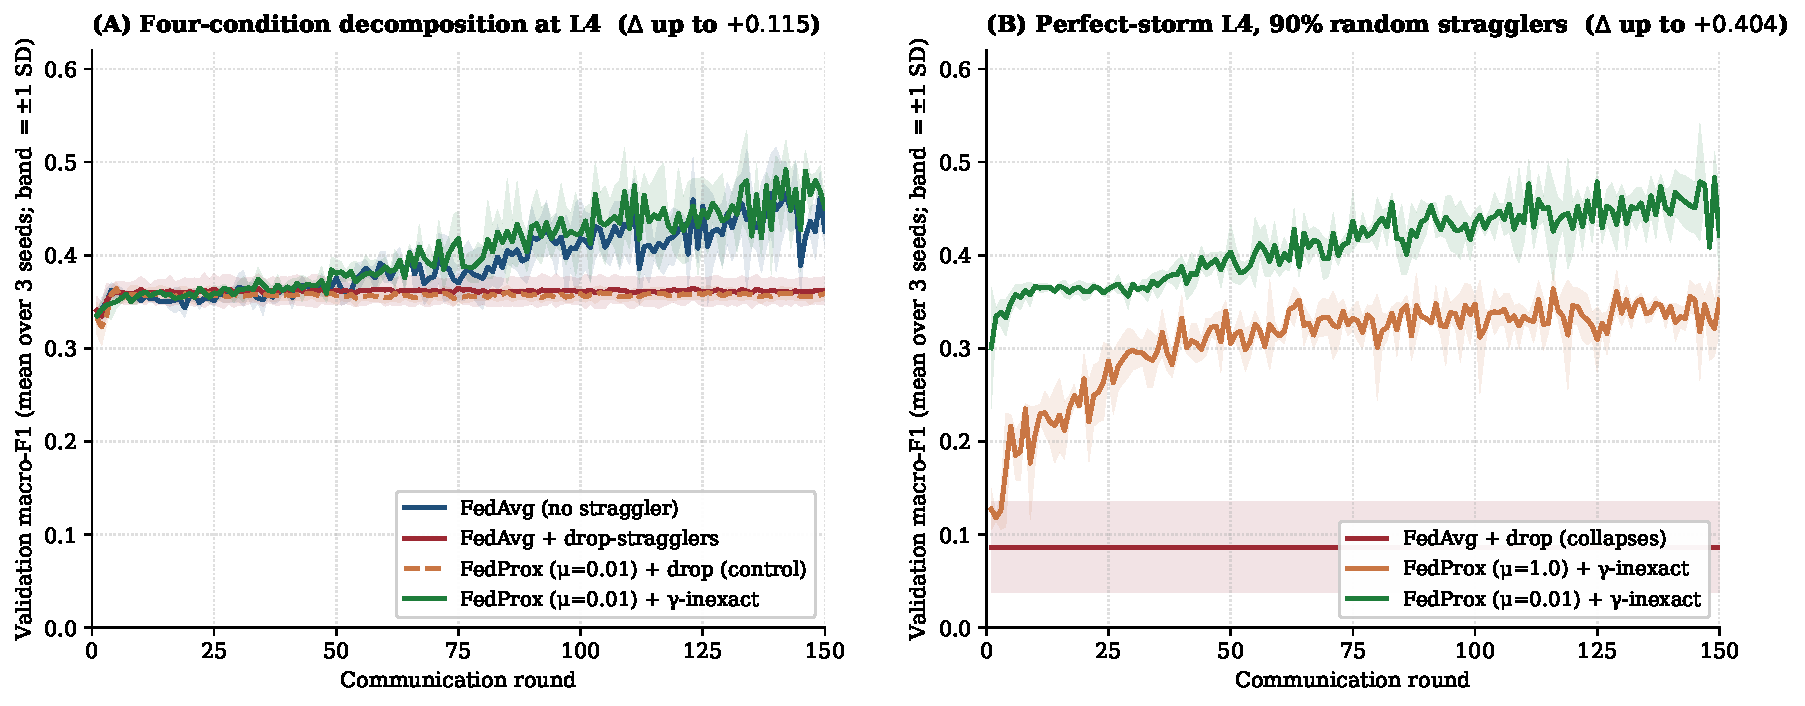
\includegraphics[width=\textwidth]{F_val_curves_extreme_gaps.pdf}
\caption{Validation macro-F1 trajectories at the two experiments showing the
largest FedAvg vs FedProx differences (mean over three seeds; bands are
$\pm 1$ SD). (A) Li 2020 §5.2 four-condition decomposition: the two
drop-handling curves overlap throughout training. (B) Perfect-storm L4 with
$90\%$ random stragglers: FedAvg+drop flatlines at $0.087$ for the entire
training run.}
\label{fig:cond-val-curves}
\end{figure}

The qualitative ordering reproduces at the literature-canonical extreme.
The perfect-storm L4 recipe \citep{li2020fedprox} --- $90\%$ random
stragglers per round, batch size $10$, no momentum --- produces a
within-pair $\Delta = +0.404$ macro-F1 between FedProx with $\mu = 0.01$
and $\gamma$-inexact ($0.491 \pm 0.003$) and FedAvg with drop
($0.087 \pm 0.049$). At $\mu = 1.0$, FedProx reaches only $0.365 \pm 0.023$,
$0.126$ below the well-tuned-$\mu$ result, consistent with the
$\mu$-sensitivity pattern of Section~\ref{sec:cond-stat-het}. Under
perfect-storm, FedAvg's validation macro-F1 is genuinely flat at $0.087$ for
all $150$ rounds (Figure~\ref{fig:cond-val-curves}B): in most rounds only the
data-dominant Client~0 contributes to the aggregation, and the global model
collapses to predicting only that client's distribution.

Figure~\ref{fig:cond-escalation} synthesises five stress conditions of
increasing severity. The within-pair $\Delta$ is essentially zero under both
IID and the L4 symmetric protocol (despite L4's JS divergence of $0.385$),
becomes substantial under the Li 2020 §5.2 straggler protocol, and grows
further under perfect-storm.

\begin{figure}[!htbp]
\centering
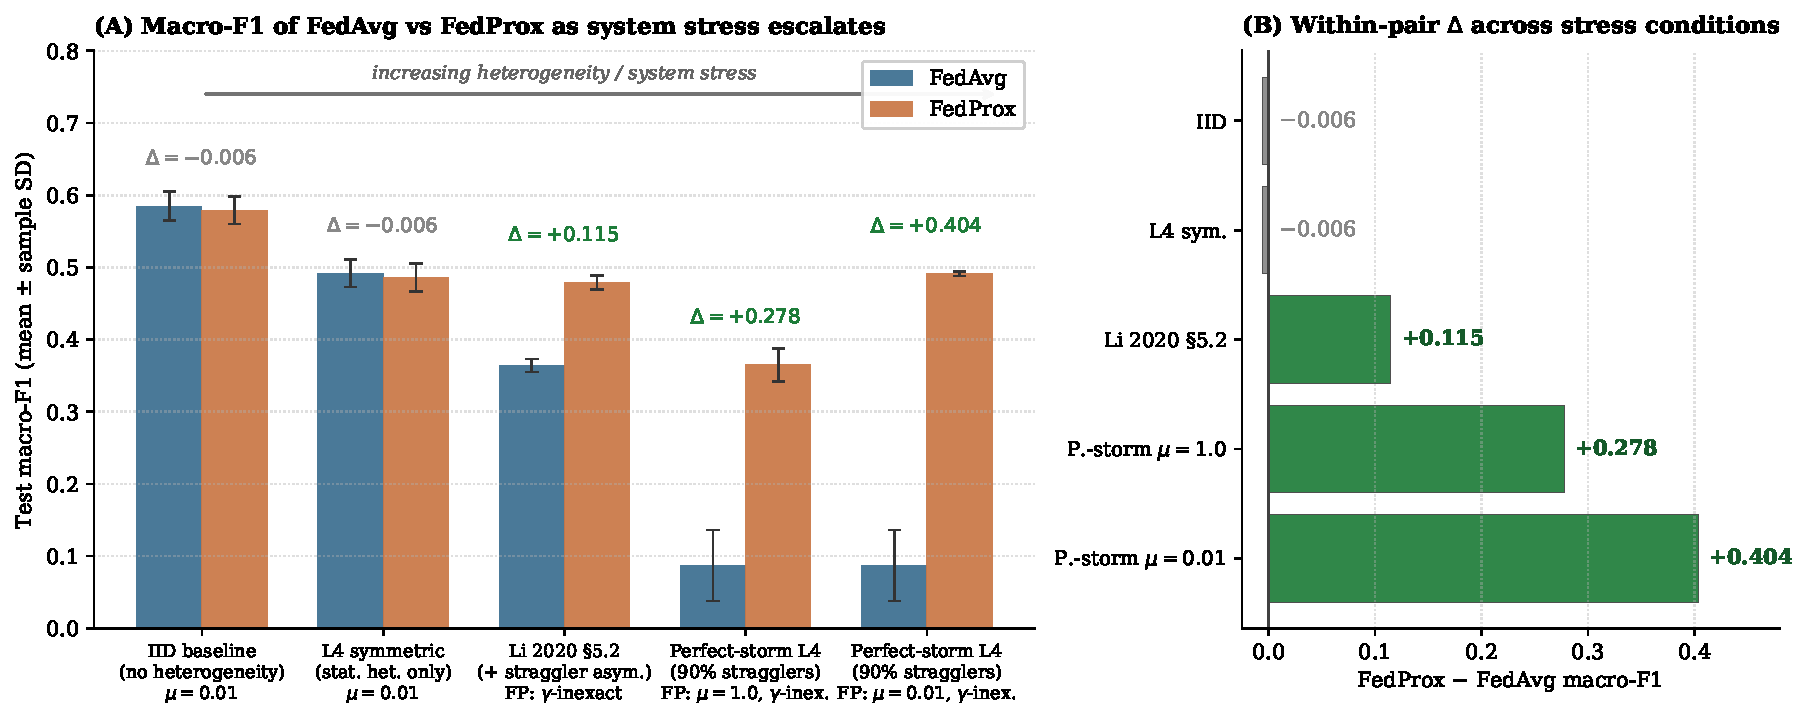
\includegraphics[width=\textwidth]{F_heterogeneity_escalation.pdf}
\caption{Heterogeneity-escalation synthesis. (A) Test macro-F1 of FedAvg vs
FedProx across five conditions of increasing system stress; error bars are
sample SD across the available seeds. (B) The within-pair $\Delta$ ordered
identically. The FedProx advantage is essentially zero under IID and
symmetric non-IID, becomes large under straggler asymmetry, and grows
further under the literature-canonical $90\%$ random-straggler regime.}
\label{fig:cond-escalation}
\end{figure}

Partial client participation ($C = 0.5$: four of seven clients sampled per
round; the engineered $7$-client partition of
Section~\ref{sec:cond-small-hospital}) produces a within-pair
$\Delta = +0.020$ macro-F1 over ten seeds, larger than the symmetric
engineered $\Delta = +0.027$ in seeds where the per-round client sets
synchronise but consistent with the directional pattern: smaller
per-round aggregation pools make the proximal regulariser empirically more
active.

\paragraph{Finding 3.}
\textit{The FedProx vs FedAvg gap is governed by system asymmetry, not by
statistical heterogeneity. The operative mechanism is $\gamma$-inexact
partial-update handling, not the proximal regulariser: under matched
drop-handling the proximal-only effect is $+0.004$, whereas under matched
proximal handling the $\gamma$-inexact effect is $+0.111$. Under the
literature-canonical $90\%$ straggler regime the gap reaches $+0.404$
macro-F1 because FedAvg fails to learn at all.}

\section{System Heterogeneity: Learning-Rate Asymmetry}
\label{sec:cond-lr-asymmetry}

A second form of system asymmetry --- different per-client effective step
sizes --- exposes a complementary failure mode. On the L4 partition we hold
$\eta_0 = 0.01$ at Client~0 and vary $\eta_1 \in \{0.01, 0.005, 0.002\}$ at
Client~1 (LR ratios $1{:}1$, $2{:}1$, $5{:}1$), giving $27$ runs
($3$ algorithms $\times 3$ ratios $\times 3$ seeds). Test macro-F1 at the
endpoints is reported in Table~\ref{tab:cond-lr-asymmetry}.

\begin{table}[!htbp]
\centering
\caption{Test macro-F1 under per-client LR asymmetry on L4 (3 seeds; mean
$\pm$ sample SD).}
\label{tab:cond-lr-asymmetry}
\small
\begin{tabular}{lccc}
\toprule
Algorithm & $1{:}1$ symmetric & $5{:}1$ asymmetric & $\Delta$ \\
\midrule
FedAvg                  & $0.457 \pm 0.026$ & $0.375 \pm 0.016$ & $-0.083$ \\
FedProx ($\mu = 0.01$)  & $0.491 \pm 0.016$ & $0.392 \pm 0.017$ & $-0.099$ \\
\textbf{FedNova}        & $\mathbf{0.509 \pm 0.016}$ & $\mathbf{0.504 \pm 0.007}$ & $\mathbf{-0.006}$ \\
\bottomrule
\end{tabular}
\end{table}

FedAvg and FedProx degrade by $0.083$ and $0.099$ macro-F1 respectively under
$5{:}1$ LR asymmetry; FedNova degrades by only $0.006$, within seed noise.
The mechanism is FedNova's $\tau_i$-normalisation: under $5{:}1$, the ratio of
Client~1's mean update norm to its $1{:}1$ baseline is $0.47$ for FedAvg and
$0.50$ for FedProx (approximately proportional to its learning-rate
reduction), but $0.91$ for FedNova. The smaller client's effective
contribution is approximately preserved under FedNova while it is attenuated
under FedAvg and FedProx. The proximal term provides no protection here ---
FedProx degrades marginally more than FedAvg, not less.

The same algorithm, however, fails catastrophically under the regime it was
designed for. A single-seed pilot of FedNova under unequal-$E$
($E_0 = 20, E_1 = 5$) on L3 and L4 reports the drops in
Table~\ref{tab:cond-fednova-unequal-e}. FedAvg and FedProx degrade modestly
($\Delta_E$ of $-0.003$ to $-0.058$); FedNova drops $-0.224$ at L3 and
$-0.192$ at L4 between equal-$E$ and unequal-$E$. The $\tau_i$-normalisation
that protects against LR asymmetry amplifies noise from the small-batch
straggler under non-IID at the unequal-$E$ regime, contrary to the design
intent of \citet{wang2020fednova}.

\begin{table}[!htbp]
\centering
\caption{Test macro-F1 at L3 and L4 under equal-$E$ versus unequal-$E$
($E_0 = 20, E_1 = 5$); single-seed pilot.}
\label{tab:cond-fednova-unequal-e}
\small
\begin{tabular}{llccc}
\toprule
Partition & Algorithm & Equal-$E$ & Unequal-$E$ & $\Delta_E$ \\
\midrule
L3 & FedAvg            & $0.511$ & $0.508$ & $-0.003$ \\
L3 & FedProx           & $0.549$ & $0.557$ & $+0.007$ \\
L3 & FedNova           & $\mathbf{0.535}$ & $\mathbf{0.310}$ & $\mathbf{-0.224}$ \\
L4 & FedAvg            & $0.482$ & $0.424$ & $-0.058$ \\
L4 & FedProx           & $0.478$ & $0.452$ & $-0.026$ \\
L4 & FedNova           & $\mathbf{0.522}$ & $\mathbf{0.330}$ & $\mathbf{-0.192}$ \\
\bottomrule
\end{tabular}
\end{table}

\paragraph{Finding 4.}
\textit{Learning-rate asymmetry and computational-work asymmetry expose
algorithms differently. FedNova preserves macro-F1 under LR asymmetry but
collapses under unequal local-epoch counts; FedAvg and FedProx are
symmetric in the opposite direction. The optimiser ranking is
heterogeneity-type-dependent.}

\section{Per-Class Failure Mode: Rare-Class Collapse}
\label{sec:cond-rare-class}

Macro-F1 understates the clinically relevant per-class consequences of
optimiser failure. Across $91$ L4 runs spanning fourteen experimental
conditions, the row-normalised confusion-matrix diagonal shows a
qualitatively consistent failure mode: when a federated optimiser fails on
this benchmark, rare-class inputs are not randomly misclassified but are
predominantly assigned to the majority class (mel-nevi, $66.9\%$ of the
test set). Figure~\ref{fig:cond-rare-heatmap} reports the diagonal across
fourteen protocols.

\begin{figure}[!htbp]
\centering

\includegraphics[width=\textwidth]{F_l4_diagonal_heatmap.pdf}
\caption{Per-class test accuracy across fourteen L4 protocol configurations.
Yellow lines bracket the three lower-support rare classes (dermatofibroma,
melanoma, vascular). Cells with accuracy $< 0.1$ indicate near-total failure
on the corresponding class.}
\label{fig:cond-rare-heatmap}
\end{figure}

The fraction of true rare-class test inputs (dermatofibroma, melanoma,
vascular) predicted as mel-nevi ranges from $24\%$ at the heterogeneity-
ladder protocol to $67\%$ under the perfect-storm FedAvg+drop protocol.
Misrouting exceeds $50\%$ under: FedAvg+drop in the Li 2020 §5.2 protocol
($56\%$), FedAvg+drop in perfect-storm ($67\%$), FedProx $\mu = 1.0$ in
perfect-storm ($54\%$), and FedAvg under $5{:}1$ LR asymmetry ($51\%$).
Melanoma is the most clinically critical and best-resolved rare class
(test support $n = 223$ versus $n = 23$ for dermatofibroma and $n = 29$
for vascular); under $5{:}1$ LR asymmetry, melanoma detection
(row-normalised diagonal) is $1.2\%$ under FedAvg, $6.1\%$ under FedProx,
and $46.3\%$ under FedNova.

\begin{figure}[!htbp]
\centering

\includegraphics[width=\textwidth]{F_l4_confusion_d1_5_1.pdf}
\caption{Row-normalised confusion matrices at L4 contrasting the $1{:}1$
symmetric baseline (top row) with the $5{:}1$ learning-rate asymmetric
condition (bottom row) across the three algorithms. Yellow rectangles mark
the rare-class rows.}
\label{fig:cond-confusion-d1}
\end{figure}

Rare-class collapse, when it occurs, follows one of two qualitatively
distinct trajectories. Under drop-handling protocols (Li 2020 §5.2,
perfect-storm), rare-class F1 falls to zero within the first one to two
communication rounds: the collapse is \emph{instantaneous}, caused by the
rare-class-holding Client~1 being dropped from aggregation. Under
learning-rate asymmetry, rare-class F1 decays over tens of rounds: the
collapse is \emph{gradual}, caused by the high-learning-rate Client~0
progressively overwhelming Client~1's preserved-but-reduced contribution.
Both modes are detectable from round $20$ alone. A multivariate
logistic-regression classifier on twelve per-class F1 features at round
$20$ predicts final-round collapse with cross-validated AUC $= 0.844$
($n = 76$ training, $18$ positive); on an independent prospective held-out
set ($n = 12$, $1$ positive) all twelve runs are flagged correctly.

\paragraph{Finding 5.}
\textit{Federated-optimiser failure on this benchmark is directional, not
random: rare-class inputs collapse into mel-nevi. The collapse exhibits two
distinct trajectories (instantaneous under drop-handling, gradual under
learning-rate asymmetry) and is detectable from round 20 with
cross-validated AUC $0.844$.}

\section{Mechanism: Per-Client Update Norms}
\label{sec:cond-mechanism}

The aggregate per-client update norm $\Vert \Delta w_k^{(t)} \Vert_2$,
averaged over $150$ rounds, provides exploratory mechanism evidence.
Figure~\ref{fig:cond-update-norms} shows the engineered-partition norms for
the headline ten-seed experiment.

\begin{figure}[!htbp]
\centering
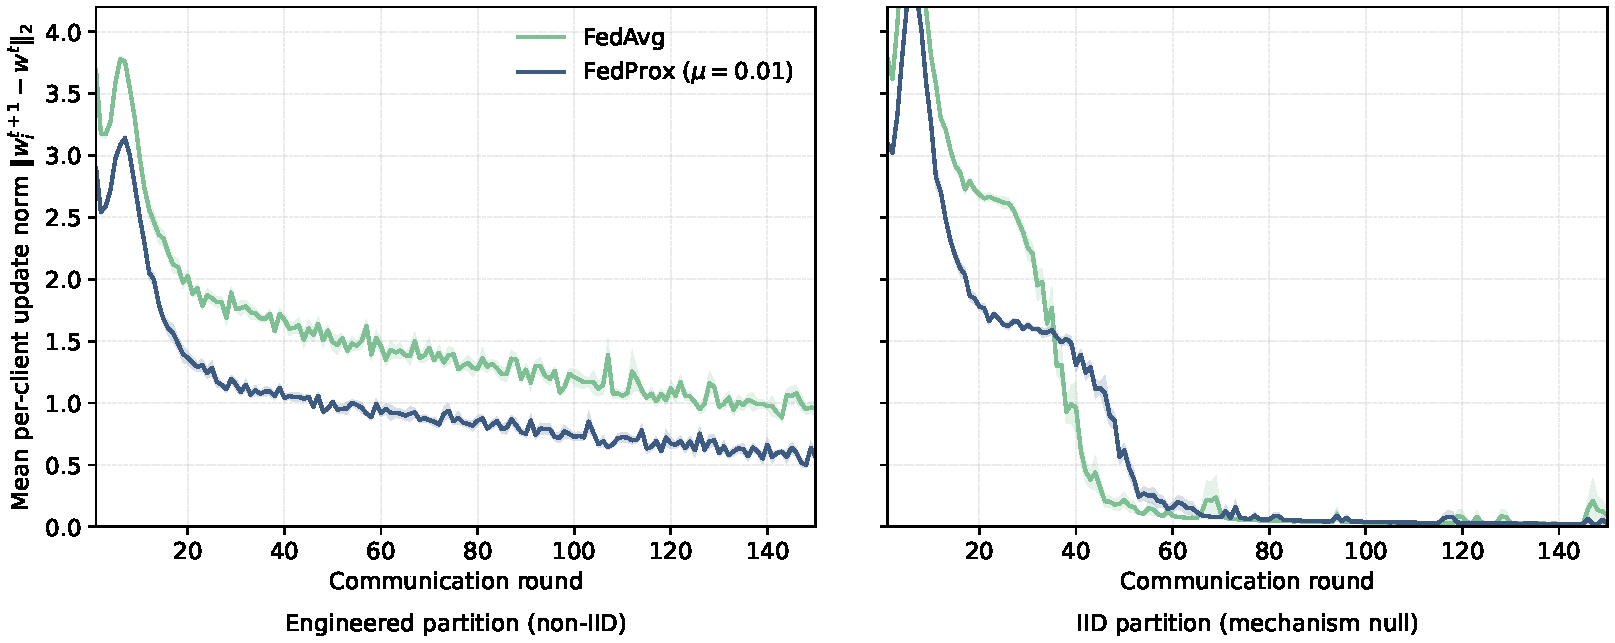
\includegraphics[width=0.95\textwidth]{F_update_norms.pdf}
\caption{Per-client mean update norms across rounds on the engineered
partition (mean over ten seeds; shading is $\pm 1$ SD).}
\label{fig:cond-update-norms}
\end{figure}

Client~1, the rare-class holder, produces consistently larger update norms
than Client~0 across both algorithms ($\Vert \Delta w_1 \Vert / \Vert
\Delta w_0 \Vert = 3.49$ for FedAvg and $3.63$ for FedProx), reflecting its
higher per-round local loss. The proximal term does not visibly suppress
this ratio; instead, FedProx slightly amplifies the dominant-client
contribution while modestly reducing trajectory volatility.

Across $78$ L4 runs spanning eight experimental conditions, the within-
protocol ordering of Client~1's relative influence does not extrapolate to
the cross-protocol pattern. The Spearman correlation between the
Client-1/Client-0 influence ratio and final rare-class F1 is $r = +0.80$
within the LR-asymmetry experiment alone for FedAvg ($r = +0.87$ for
FedProx) but is essentially zero ($r = -0.04$) when pooling across the
eight protocols. The strongest cross-protocol predictor of rare-class F1 is
the absolute magnitude of Client~0's mean update norm: $r = +0.63$ across
all $78$ runs. Rare-class preservation tracks the dominant client's update
activity, not the rare-class client's relative influence.

\paragraph{Finding 6.}
\textit{Across $78$ L4 runs spanning eight protocols, the dominant client's
mean update-norm magnitude is the strongest cross-protocol predictor of
rare-class F1 ($r = +0.63$), while the relative-influence ratio is not
($r = -0.04$ across protocols). Rare-class learning paces with the
dominant client's update activity rather than with the rare-class client's
share of the aggregation.}

\section{Algorithmic Ablations and Methodological Audits}
\label{sec:cond-ablations}

\paragraph{Class-weighted CE compositionality.}
A $2 \times 2$ factorial of FedAvg/FedProx $\times$ standard/weighted CE
on L4 (3 seeds per cell) gives loss-effect $+0.029$ macro-F1,
algorithm-only effect $\approx 0$, combined effect $+0.027$, and
interaction $-0.004$. The two interventions are essentially additive, but
the algorithm-only effect (FedProx vs FedAvg under weighted CE) collapses
to near-zero --- FedProx adds no meaningful improvement on top of
weighted-CE loss-side rebalancing in the symmetric regime.

\paragraph{Asymmetric per-client $\mu$.}
A directional test motivated by Yao~$2024$ assigns the proximal anchor to
only the dominant client (Anchor-large, $\mu_0 = 0.01, \mu_1 = 0$) or only
the rare-class-holding client (Anchor-small, $\mu_0 = 0, \mu_1 = 0.01$).
Anchor-large reaches $0.495 \pm 0.029$ and Anchor-small reaches
$0.464 \pm 0.008$, giving a direction effect of $+0.032$ macro-F1 ---
approximately $1.6$ pooled cross-condition standard deviations. The
directional prescription is not supported on this benchmark in the
direction predicted.

\paragraph{Reporting-protocol robustness.}
Test macro-F1 read at best-validation, final-round, and last-$25$-round
mean yields different algorithm orderings for some experiments. Across the
six multi-seed experiments in this chapter, $0/9$ seed-level comparisons
flip on the three large-effect experiments (mean $|\Delta| \geq 0.04$:
perfect-storm, Li 2020 §5.2, asymmetric $\mu$) and $4/9$ flip on the three
small-effect experiments (mean $|\Delta| < 0.04$: engineered baseline,
extended-rounds L3, node-pinned L4). Reporting-protocol flips track effect
magnitude: large effects are reporting-robust; small effects are not.

\paragraph{Training stability across algorithms.}
The standard deviation of validation macro-F1 over the last $50$ rounds of
training, pooled across all runs in this chapter, is $0.024$ for FedAvg
symmetric, $0.019$ for FedProx symmetric, and $0.048$ for FedNova symmetric;
the FedNova end-of-training instability is approximately $2.0\times$ the
FedAvg value. Under unequal-$E$ the corresponding values are $0.020$,
$0.028$, and $0.060$ (FedNova $3.0\times$ FedAvg). FedNova is the most
oscillation-prone algorithm in steady state, consistent with the
unequal-$E$ failure of Section~\ref{sec:cond-lr-asymmetry}.

\paragraph{B-dissimilarity proxy.}
The empirical proxy for the Li 2020 $B$ parameter (mean ratio of maximum
to mean per-client update norm at FedAvg, averaged over $150$ rounds,
three seeds) increases monotonically with heterogeneity (Spearman
$r = +0.90$ vs Jensen--Shannon divergence). The FedProx-versus-FedAvg
within-pair $\Delta$ correlates only weakly and negatively with this
empirical $B$-proxy ($r \approx -0.30$ across the five ladder partitions):
the partitions at which the theoretical predictor says FedProx should help
most are the partitions where FedProx helps least. We do not present this
as a refutation of the Wang--Li bound under its smoothness assumptions,
but the simple $B$-proxy is not a useful practitioner heuristic on this
benchmark.

\section{Small-Hospital Case Study}
\label{sec:cond-small-hospital}

A seven-client case study examines the federation-value contrast in the
canonical small-hospital regime: six large clients hold the common classes,
one small client holds only the rare classes (dermatofibroma, melanoma,
vascular). Trained alone on its local data, the small client reaches a
mean macro-F1 of $0.183$; trained centrally on the pooled training set, it
reaches $0.560$. Under FedAvg the small client receives a global model
worth $0.395$ macro-F1, a $+0.212$ gain over local-only training, and
under FedProx ($\mu = 0.01$) it receives $0.417$, a $+0.234$ gain. The
case study is reported on a single seed and is not used as a quantitative
contribution; the qualitative claim is that the rare-class-holding
participant gains substantially from federation, and slightly more from
FedProx than from FedAvg.

\section{Summary of Findings}
\label{sec:cond-summary}

Table~\ref{tab:cond-summary} summarises FedAvg vs FedProx (and FedNova
where tested) across the principal heterogeneity scenarios of this
chapter.

\begin{table}[!htbp]
\centering
\caption{Summary of FedAvg vs FedProx (vs FedNova where tested) across
heterogeneity scenarios. All entries are test macro-F1; $\Delta$ is the
within-pair FedProx $-$ FedAvg. Seed counts vary; see referenced sections.}
\label{tab:cond-summary}
\small
\begin{tabular}{llrrrr}
\toprule
Heterogeneity & Protocol  & FedAvg  & FedProx & FedNova & $\Delta_{\mathrm{FP-FA}}$ \\
\midrule
None               & Centralised baseline (10 s) & $0.560$ & ---     & ---     & ---       \\
None               & IID federated (10 s)        & $0.585$ & $0.579$ & ---     & $-0.006$  \\
Statistical only   & Engineered 90/10 (10 s)     & $0.477$ & $0.503$ & ---     & $+0.027$  \\
Statistical only   & Dirichlet $\alpha = 0.1$ (10 s) & $0.480$ & $0.488$ & ---     & $+0.008$  \\
Statistical only   & Heterogeneity ladder L4 (1 s) & $0.518$ & $0.492$ & $0.506$ & $-0.026$  \\
Statistical only   & Node-pinned L4 (3 s)        & $0.492$ & $0.486$ & ---     & $-0.006$  \\
Stat. + system     & Li 2020 §5.2 4-cond. (3 s)  & $0.364$ & $0.479$ & ---     & $+0.115$  \\
Stat. + system     & Perfect-storm L4 (3 s)      & $0.087$ & $0.491$ & ---     & $\mathbf{+0.404}$ \\
Stat. + LR asym.   & D1 5:1 ratio (3 s)          & $0.375$ & $0.392$ & $\mathbf{0.504}$ & $+0.017$ \\
Stat. + unequal-E  & Unequal-$E$ L4 (1 s)        & $0.424$ & $0.452$ & $0.330$ & $+0.028$ \\
Loss intervention  & Weighted-CE on L4 (3 s)     & $0.505$ & $0.503$ & ---     & $-0.002$  \\
\bottomrule
\end{tabular}
\end{table}

The six findings restate as a single coherent picture. Statistical
heterogeneity alone is insufficient to separate the algorithms under
matched symmetric protocols (Finding $2$): the engineered partition's
$\Delta = +0.027$ is real but small, and the node-pinned L4 multi-seed
result is null. System asymmetry --- specifically asymmetric stragglers ---
opens the gap by an order of magnitude (Finding $3$), but the responsible
mechanism is $\gamma$-inexact partial-update handling and not the proximal
regulariser that names FedProx (Finding $3$, four-condition
decomposition). A second form of system asymmetry, learning-rate
asymmetry, reverses the algorithm ranking in FedNova's favour (Finding
$4$), although the same FedNova fails catastrophically under the
unequal-local-epoch regime it was designed to address. Across all
failure modes the per-class signature is the same: rare-class inputs
collapse into the majority class, in one of two distinct trajectories that
are detectable from round 20 (Finding $5$). The cross-protocol mechanism
correlate is the dominant client's update-norm magnitude, not the rare-
class client's influence ratio (Finding $6$).

The practical guidance from this study is therefore narrower than the
literature suggests. Under matched data and symmetric compute, FedAvg is
sufficient. Under asymmetric stragglers, FedProx is valuable, but the
empirical value comes from accepting partial updates rather than from
adding a proximal anchor. Under learning-rate asymmetry, FedNova is the
robust choice. The proximal-coefficient $\mu$ has a narrow operating
range: small ($\mu \leq 0.01$) on this benchmark, and large $\mu$ is
actively harmful at every heterogeneity level tested.

\section{Limitations}
\label{sec:cond-limitations}

The empirical scope of these findings is restricted to a single dataset
(DermaMNIST $28 \times 28$, seven classes, $66.9\%$ majority class), a
small CNN ($\sim 100$k parameters with GroupNorm), a two-client federation
(with one seven-client case study), $E = 20$ local epochs, and SGD with
momentum $0.9$. The magnitude of the FedProx-vs-FedAvg gap is expected to
grow with larger $E$ (more local drift to constrain) and with adaptive
optimisers (more local-overfitting potential); these regimes are not
tested here. Single-seed pilot results are explicitly marked as such; the
multi-seed promotions use three or ten seeds per cell, and the headline
Wilcoxon claim uses paired-seed protocol on ten seeds.

\bibliographystyle{plainnat}
\bibliography{mnist_dermnist/results/thesis_ready/writing/references}

\end{document}
